\documentclass[titlepage,landscape]{seminar}
\usepackage{url}
\usepackage{graphicx}
\usepackage[pdftex]{color}
\usepackage{hyperref}
\usepackage{epstopdf}
\usepackage{slides}

\newcommand{\frack}{\frac{1}{k}}

\begin{document}

\myslide{
\begin{center}
\begin{tabular}{c|ccc}
\hline\hline
Method & $F_{is}$ & $F_{st}$ \\
\hline
Direct            & 0.14 & 0.21 & 0.32 \\
Nei               & 0.31 & 0.24 & 0.47 \\
Weir \& Cockerham & 0.54 & 0.04 & 0.56 \\
Bayesian          & 0.53 (0.33, 0.70) & 0.11 (0.02, 0.22) \\
\hline
\end{tabular}
\end{center}
}

\myslide{
\begin{eqnarray*}
\mbox{P}(i|k) &=& \frac{\mbox{P}(x_i|\gamma_k)}{\sum_k
  \mbox{P}(x_i|\gamma_k)} \\
x_i &=& \mbox{genotype of individual $i$} \\
\gamma_k &=& \mbox{genotype frequencies in population $k$}
\end{eqnarray*}
For example, if $A_1A_1$ is labeled as $1$, $A_1A_2$ as $2$, $A_2A_2$
as 3, and we assume that genotypes are in Hardy-Weinberg, then
\begin{eqnarray*}
\mbox{P}((1,2,2,1,3)|(p_{k1}, p_{k2}, p_{k3}, p_{k4}, p_{k5})) = (p_{k1}^2)(2p_{k2}q_{k2})(2p_{k3}q_{k3})(p_{k4}^2)(q_{k5}^2)
\end{eqnarray*}
}

\myslide{
{\it Berberis thunbergii\/}
\begin{itemize}
\item 85 feral, 7 horticultural, 4 cultivated
\item 147 polymorphic AFLP markers
\end{itemize}
\begin{table}
\begin{center}
\begin{tabular}{cc}
\hline\hline
K & Mean L(K) \\
\hline
2 & -2553.2 \\
3 & {\bf -2331.9} \\
4 & -2402.9 \\
5 & -2476.3 \\
\hline
\end{tabular}
\end{center}
\caption{Mean log probability of the data for $K=2,3,4,5$ in the {\it
    Berberis thunbergii\/} data}
\end{table}
}

\myslide{
\begin{figure}
\resizebox{\textwidth}{!}{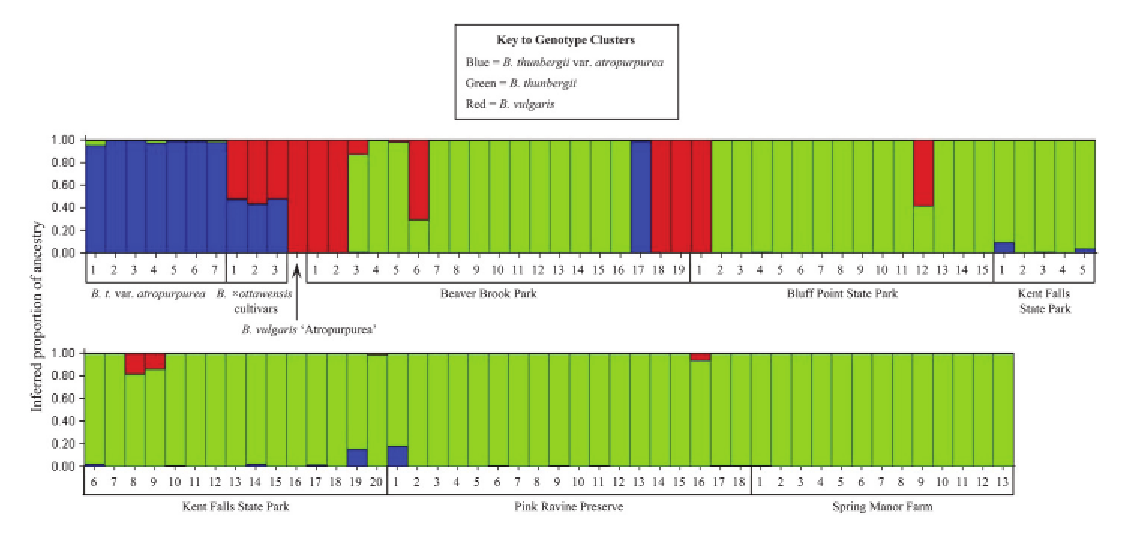
\includegraphics{lubell-structure.eps}}
\caption{Analysis of AFLP data from {\it Berberis
    thunbergii}}
\end{figure}
}

\myslide{
\begin{itemize}

\item Human Genome Diversity Cell Line Panel (HGDP-CEPH)

\item 1056 individuals, 52 geographic populations, 377 autosomal
  microsatellite loci

\end{itemize}

\begin{figure}
\resizebox{\textwidth}{!}{\includegraphics{HGDP-CEPH.eps}}
\end{figure}

}

\myslide{
\begin{itemize}

\item Principal components analysis of genotypes.

\item 3129 Europeans, 500,568 SNP loci

\end{itemize}

\begin{figure}
\begin{center}
\resizebox{0.5\textwidth}{!}{\includegraphics{human-PCA.eps}}
\end{center}
\end{figure}

}

\end{document}



\end{document}

